\documentclass[conference]{IEEEtran}
% Add the compsoc option for Computer Society conferences.
%
% If IEEEtran.cls has not been installed into the LaTeX system files,
% manually specify the path to it like:
% \documentclass[conference]{../sty/IEEEtran}

% Some very useful LaTeX packages include:
% (uncomment the ones you want to load)


% *** CITATION PACKAGES ***
%
%\usepackage{cite}
% cite.sty was written by Donald Arseneau
% V1.6 and later of IEEEtran pre-defines the format of the cite.sty package
% \cite{} output to follow that of IEEE. Loading the cite package will
% result in citation numbers being automatically sorted and properly
% "compressed/ranged". e.g., [1], [9], [2], [7], [5], [6] without using
% cite.sty will become [1], [2], [5]--[7], [9] using cite.sty. cite.sty's
% \cite will automatically add leading space, if needed. Use cite.sty's
% noadjust option (cite.sty V3.8 and later) if you want to turn this off.
% cite.sty is already installed on most LaTeX systems. Be sure and use
% version 4.0 (2003-05-27) and later if using hyperref.sty. cite.sty does
% not currently provide for hyperlinked citations.
% The latest version can be obtained at:
% http://www.ctan.org/tex-archive/macros/latex/contrib/cite/
% The documentation is contained in the cite.sty file itself.


% *** GRAPHICS RELATED PACKAGES ***
%
\usepackage{graphicx}



% *** MATH PACKAGES ***
%
%\usepackage[cmex10]{amsmath}
% A popular package from the American Mathematical Society that provides
% many useful and powerful commands for dealing with mathematics. If using
% it, be sure to load this package with the cmex10 option to ensure that
% only type 1 fonts will utilized at all point sizes. Without this option,
% it is possible that some math symbols, particularly those within
% footnotes, will be rendered in bitmap form which will result in a
% document that can not be IEEE Xplore compliant!
%
% Also, note that the amsmath package sets \interdisplaylinepenalty to 10000
% thus preventing page breaks from occurring within multiline equations. Use:
%\interdisplaylinepenalty=2500
% after loading amsmath to restore such page breaks as IEEEtran.cls normally
% does. amsmath.sty is already installed on most LaTeX systems. The latest
% version and documentation can be obtained at:
% http://www.ctan.org/tex-archive/macros/latex/required/amslatex/math/





% *** SPECIALIZED LIST PACKAGES ***
%
%\usepackage{algorithmic}
% algorithmic.sty was written by Peter Williams and Rogerio Brito.
% This package provides an algorithmic environment fo describing algorithms.
% You can use the algorithmic environment in-text or within a figure
% environment to provide for a floating algorithm. Do NOT use the algorithm
% floating environment provided by algorithm.sty (by the same authors) or
% algorithm2e.sty (by Christophe Fiorio) as IEEE does not use dedicated
% algorithm float types and packages that provide these will not provide
% correct IEEE style captions. The latest version and documentation of
% algorithmic.sty can be obtained at:
% http://www.ctan.org/tex-archive/macros/latex/contrib/algorithms/
% There is also a support site at:
% http://algorithms.berlios.de/index.html
% Also of interest may be the (relatively newer and more customizable)
% algorithmicx.sty package by Szasz Janos:
% http://www.ctan.org/tex-archive/macros/latex/contrib/algorithmicx/



% correct bad hyphenation here
\hyphenation{op-tical net-works semi-conduc-tor}


\begin{document}
%

\title{Behavioral Correlation: A new approach for clustering sensors in Wireless Sensor Networks}

% author names and affiliations
% use a multiple column layout for up to three different
% affiliations
\author{\IEEEauthorblockN{Fernando Rodrigues}
\IEEEauthorblockA{University of Fortaleza\\Fortaleza - Ceara - Brazil\\
fernandorodrigues@edu.unifor.br}
\and
\IEEEauthorblockN{Angelo Brayner}
\IEEEauthorblockA{University of Fortaleza\\
Fortaleza - Ceara - Brazil\\
brayner@unifor.br}
\and
\IEEEauthorblockN{Jose E. Bessa Maia}
\IEEEauthorblockA{State University of Ceara\\
Fortaleza - Ceara - Brazil\\
jose.maia@uece.br}}


% make the title area
\maketitle


\begin{abstract}

Sensor clustering is an efficient strategy to reduce the number of messages
transmitted to the sink in a multi-hop Wireless Sensor Network. Thus far,
grouping sensors in clusters is implemented by applying the principle of spatial
locality, which may ensure spatial correlation for data sensed by sensors within
a given area. Nonetheless, in several scenarios, sensors that are not spatially
close to each other may have similar data reading patterns.
In this work we present a new approach to cluster sensors in WSN, denoted {\it
BCWSN} (Behavioral Correlation in WSN), based on the behave of recent historical
data collected by sensors. Instead of using the spatial distance among sensors
for clustering them, the proposed approach uses the concept of behavioral
correlation to group sensors, that takes into account the concepts of difference
in magnitude and trend of the time series formed by (sinomino) the sensed data.
Furthermore, two scheduling intra-clustering methods are tested: Representative
Nodes and Cluster Heads. These techniques, which incorporate the mechanism of
behavioral correlation, are compared with each other and also with the naive
strategy (without clustering or temporal correlation) and with an approach based
on temporal correlation.
In order to validate our approach, simulations with a prototype implemented in
SinalGo have been conducted over real temperature data. Our simulation shows
that with 5\% error threshold, BCWSN can save the communication overhead by as
much as 97.72\% over naive strategy and 69.02\% over a temporal correlation
approach, besides a reduction of 45.12\% in total data sensing over the other
two approaches compared, while the RMSE remains roughly stable. Hence, we
believe that our proposal greatly increases the energy efficiency for WSNs, with
little loss of accuracy.

% The results point to gains of up to 97.72\% over naive strategy in terms of
% reduction in message transmission and 45,12\% of reduction in data sensing,
% while the RMSE remains roughly stable. To the best of our knowledge, we believe
% that our proposal brings gains in energy efficiency for WSNs.

% The best way to improve prediction accuracy is by decreasing prediction errors,
% using the same energy amount than the second version, but there is a trade-off
% between prediction accuracy and energy consumption.

\end{abstract}

% IEEEtran.cls defaults to using nonbold math in the Abstract.
% This preserves the distinction between vectors and scalars. However,
% if the conference you are submitting to favors bold math in the abstract,
% then you can use LaTeX's standard command \boldmath at the very start
% of the abstract to achieve this. Many IEEE journals/conferences frown on
% math in the abstract anyway.

% no keywords




% For peer review papers, you can put extra information on the cover
% page as needed:
% \ifCLASSOPTIONpeerreview
% \begin{center} \bfseries EDICS Category: 3-BBND \end{center}
% \fi
%
% For peerreview papers, this IEEEtran command inserts a page break and
% creates the second title. It will be ignored for other modes.
\IEEEpeerreviewmaketitle



\section{Introduction}
% no \IEEEPARstart


Sensors are devices used to collect data from the environment related to the
detection or measurement of physical phenomena. Sensors are limited in power,
computational capacity, and memory. Advances in wireless communication have
enabled the development of massive-scale wireless sensor networks (WSN). In a
WSN, sensors are usually scattered in the network and use low-power
communication channels. Thus, sensors disseminate collected data to a base
station, from where the information (query) was originally requested. Wireless
sensor networks (WSNs) have been widely used for environmental monitoring (e.g.,
traffic, habitat), industrial sensing and diagnostics (e.g., factory, supply
chains), infrastructure protection (e.g., water distribution), battlefield
awareness (e.g., multi-target tracking) and context-aware computing (e.g.,
intelligent home) applications.


%WSNs can be categorized into three types, depending on the application or the
%use pattern of the network. Thus, there exist WSNs for: {\it (i)} responding to
%user queries \cite{Brayner2007}; {\it (ii)} continuously sensing (stream), or;
%{\it (iii)} monitoring of certain sporadic events \cite{Ren2007}. These uses are
%not mutually exclusive, i.e. in a WSN that responds to queries, one can submit
%queries to request data to be sensed with a certain frequency (continuous
%sensing) and even data whenever certain events occur. The case that stands out
%as being the most critical usage is exactly the continuous sensing, because, in
%this case, every certain time interval programmed, the sensor nodes need to take
%readings and send the values read through the network, passing from node to
%node, until these data reach the sink \cite{Villas2012}.


In spite of advances in WSN technology, a critical key point is still the
energy consumption of sensor nodes. It is well known that communication among
sensors is the activity responsible for the bulk of the power consumption. By
reducing communication costs, energy may be drastically saved, consequently
increasing the WSN's lifetime. An effective strategy to reduce energy
consumption is thus to reduce the number of messages (sensed data) sent across
the network. Nevertheless, the less the number of sensed data is transmitted,
the lower the accuracy of results provided by a WSN is. Thus higher accuracy in
WSNs comes at a higher energy cost.

By now, it is well-known that data collected by WSN are strongly temporally
and/or spatial correlated \cite{Yoon2005, Chu2006}. The traditional spatial data
correlation is related to the idea that the physical proximity among sensors
leads to similar measurements (values) of sensed data, phenomenon known as
"principle of spatial locality". Thus, one can infer that from the capture of
some sensors readings (located in some regions of sensing space), it is possible
to obtain, approximately, the values of the readings of other sensors in its
surroundings. On the other hand, the temporal correlation indicates the various
readings of a sensor within a time interval have a certain approximation of
their values (principle of temporal locality). such a feature makes possible to
predict (with a certain margin of error) sensed values in the future based on
data collected in the past.


Grouping sensors in clusters is the main technique used to take advantage of the
principle of spatial locality for reducing the energy consumption in WSNs. This
is because one can use only a few representative nodes from each cluster to
sense data in a given spatial region (cluster) in which sensors are spatially
correlated.
Several works have been proposed in order to use that technique, with different
approaches \cite{Chu2006, Villas2012, Singh2010, Liu2007, Shah2007}.

%In continuous environmental monitoring applications the sensors in a dense WSN
%generate a data stream that must be transmitted to a Sink to be processed and
%stored in a Fusion and Decision Center (FDC). It is widely noted [x, x, x] that
%this data stream exhibits strong spatio-temporal correlation.

Nonetheless, in several scenarios sensors, which are not spatially close to each
other, may have similar data reading patterns. In order to illustrate such a
claim consider a dense WSN deployed to monitor forest fires. 
%in which a magnitude of temperature is monitored.
Now, suppose a scenario in which the monitored region is affected by dozens of
small forest fires. Figure \ref{fig:contour_lines} depicts a possible temperature
contour lines graph for this hypothetical situation. Observe that the contour
lines in Figure \ref{fig:contour_lines} form several closed regions representing
areas which may have small forest fire areas, where it is very likely that the
temperature measurements of sensors in those spatially separated regions present
high correlation. For that reason, we claim that in such cases, a better
alternative would be to use sensor clustering strategy based on
\textit{Behavioral Correlation}.

The idea behind the concept of {\it Behavioral Correlation} is to identify
similar patterns of sensor readings even in sensors which are geographically
distant from each other. Thus, one could apply a Behavioral Correlation
Clustering (BCC) technique to group sensors which are spatially separated into a
single cluster, in contrast to existing spatio-temporal correlation techniques.
The BCC technique clusters sensors for which the forecasting models of sensed
data time series are approximately the same independent of spatial proximity of
sensors.

%Note that the BCC naturally captures the spatial grouping, if it
%exists, since the correlation is between the sensor time series. Several
%measures of similarity, dissimilarity or statistical correlation can be used to
%group the sensors based on the its time series. Also, several strategies can be
%used to trigger the evaluation of clustering: periodic, sliding windows,
%triggering threshold and others.

%Note that behavioral correlation clustering (BCC) is enabled by centralized
%clustering, being more difficult to implement in distributed correlation or
%clustering approaches, among other things, due to the limited range of sensor
%transmissions.

%\begin{figure}[!htb]
%\centering
%	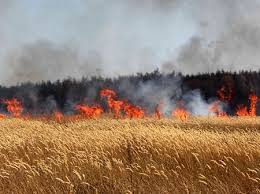
\includegraphics[scale=0.7]{I1.png}
%    \caption{Forest fire photography}
 %   \label{lab}
%\end{figure}

\begin{figure}[!htb]
\centering
	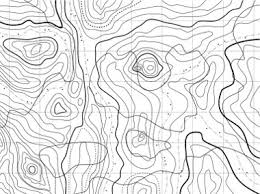
\includegraphics[scale=0.7]{I2.png}
    \caption{Contours lines of temperature}
    \label{fig:contour_lines}
\end{figure}

In this sense, in this paper, we present new approach for clustering sensors in
WSNs. The main features of the proposed approach are: {\it (i)} Cluster
formation based on the \textit{Behavioral Correlation} of the sensors, which, in
turn, is computed from the time series of sensor readings by applying a
\textit{Similarity Measure}, and; {\it (ii)} the use of a linear regression
model for the temporal suppression of sensed data through the maximum error
level (threshold) desired by the user used to control the data to be sent to the
sink. Furthermore, two different approaches to select of active nodes
(scheduling) in each cluster have been implemented: Representative Nodes (RNs)
and Cluster Heads (CHs).

Hence, special sensor nodes only transmit data which are novelties for the
regression model applied by our propose.

% Another way to reduce the energy consumption of a sensor network, thereby
% increasing the its lifetime, is using the principle of temporal locality
% \cite{MaiaSAC2013}.
% In this way, in an external environment, without artificial interventions, most
% of the time, one can predict the values to be measured by the sensors with a
% certain margin of error from a history of readings and with the application of a
% regression model
%  \footnote{Several studies have proposed the use of this
% technique, taking advantage of predictions across both time and space, with
% different approaches.} (e.g.: linear, like $\bar{S}(t) = A + B(t)$).

% Furthermore, two different approaches to the way of selection of active nodes
% (scheduling) in each cluster were implemented: Representative Nodes (RNs) and
% Cluster Heads (CHs).

The remainder of this document is organized as follows. [To be described\ldots]


\section{Related Work}

In \cite{Vuran2004}, proposes a strategy to cluster sensors in WSNs. The idea is
the following: given a set of N sensors, M nodes, with $M < N$, are chosen to
send data. The M representative nodes are defined based on the application of a
distortion function ($D(M)$) on sensed data.
The spatial distance between the nodes (representative) directly influences the
computation of the distortion function by means of a correlation coefficient.
That work does not take into account the energy capacity of each node as a
criterion for choosing representative nodes, although this is a very important
factor due to the restrictive characteristics regarding the energy consumption
of the nodes in a WSN.

In EAST \cite{Villas2012}, sensors are grouped into two levels, under a spatial
correlation approach, while the leader and the representative nodes perform a
temporal suppression technique.
The leader node generates a representative value for each cluster based on data
received by the representative nodes, which form a subset of all the nodes that
sense the same event. The sensed area is divided into "event areas", which in
turn are divided into "correlation regions (c) or cells", where the formers will
be managed, each one, for a "Coordinator node" and the "correlation areas" will
be represented, one by one, by a "Representative node" because a single reading
within this region is enough to represent it.
The size of the correlation region (c) can be decremented or incremented by the
sink according to the application and the characteristics of the event, to
maintain the accuracy of the data collected.

Another way to group sensor nodes into clusters is through measures of
dissimilarity.
In EEDC \cite{Liu2007}, such measures of dissimilarity are calculated by the
sink node for all pairs of nodes of the network, regardless of their location.
The measure of dissimilarity between two nodes is calculated based on up to $3$
parameters, namely:
the differences in magnitude (\textit{M}) and trend (\textit{T}) of the data
values and the geographical/euclidean distance between nodes ($g_{max}dist$).
The criterion of formation of clusters is based on the maximum threshold of
dissimilarity (max\_dst) defined by a tuple (\textit{M}, \textit{T},
$g_{max}dist$), based on the measure of dissimilarity between the nodes. It
works as follows: $1)$ Initially, the data sensed by each node are sent in the
form of a temporal series for the sink. $2)$ The sink then stores all the data
from the sensors and then calculates the measure of dissimilarity (previously
mentioned) for each pair of nodes of the network. $3)$ With the measures
calculated and the maximum threshold of dissimilarity (max\_dst), the sink
divides the nodes into clusters. The sink monitors large variations within a
cluster and dynamically adjusts the cluster in response to the changes in
spatial correlation.
The sink node recalculates the dissimilarity of active sensor nodes (pair to
pair) within each group, at the end of each time interval (time slot), after
having collected the latest samples of each active sensor node. The current
cluster must be divided if the sink node verify that there is at least one
active sensor node reporting significantly different data (i.e. outside the
max\_dst threshold with other nodes in the same cluster).
For computational reasons, it always takes into account the maximum distance
between the sensors in the calculation of dissimilarity measures.
That work does not takes into account the energy reserve of each node as a
criterion for choosing representative nodes (it is used an algorithm that makes,
simultaneously, the equitable scheduling - round robin - along with the random
choice of representatives nodes).
Furthermore, the proposal does not deal with the partial reassembly (formation
of new clusters from the union of other existing ones) of the nodes that have a
low dissimilarity (i.e. high similarity), since this measure could result in a
greater energy saving for the nodes of the network.

The spatial correlation through the formation of clusters is addressed in
\cite{Pham2010} in the form a flooding algorithm where the sink node starts to
send messages to the other nodes of the network, inviting them to form groups
from criteria such as a dissimilarity measure, in addition to the physical
proximity between nodes, since, of course, the message forwarding in a WSN
occurs between adjacent nodes (i.e. geographically close). Cluster Heads (CHs)
are selected, basically, by 2 parameters: {\it (i)} the nodes that are one hop
from the ancestor that sent the message calculate the measure of dissimilarity
with the mean value informed in the message and then those that are within the
threshold of dissimilarity if they apply for CH, where {\it (ii)} it is said to
be the CH the one that have higher level of energy reserve.
We should notice that, during the process of forming clusters, the nodes that
will form the communication backbone between each Cluster Head node and the sink
are also configured. A scheduling of each cluster is done through round robin in
order to decide which member node that will be active in each time slot making
the sensing and sending the data to its respective CH.
Each cluster has a CH and a Gateway (GW), which connects that cluster to the
neighbor cluster (or with the sink node), in the first case through a Cluster
Extend (EC or EXT).
Additionally, each cluster can obviously have several members (MEM) and also
several EC's.
The process of cluster split (formation of new clusters) is delegated to the GW
(Gateway) of each cluster, and not the CH or the sink, which do not need to be
activated for such a task. The weak point is the process of forming clusters, in
which there is an intensive exchange of messages, scattering a significant
amount of energy from the network sensors, in addition to the process of
regrouping of nodes (merge) into new unified clusters, which is only fired by
the sink using a global approach, i.e. to the entire network, not being
predicted, thus, partial regrouping of the clusters.

In \cite{Shah2007}, the spatial correlation is explored by a mechanism called
the GSC (Gridiron Spatial Correlation), where the sensed region has a Cluster
Head that will be in the center of the region delimited by r (radius of the
monitored region), which will be divided into correlated regular regions
(quadratic), according to the spatial density level chosen, defined through
$\theta$ (size of the correlation region equal to $\theta^2$). In this way,
active sensors will be chosen according to 2 basic parameters: {\it (i)} the
proximity of the them regarding the center of the regions correlated and {\it
(ii)} their energy level must be within a certain threshold, above the ones of
their closest neighbours. The scheduling of active nodes works through the
passage of a list by the cluster-head for all nodes (active and inactive, the
latter being momentarily enabled only to receive the list) with the nodes being
active in each time slot, where this configuration is only changed when one of
the active nodes has its energy level below the threshold established. Although
this solution considers the energy level of the nodes in the choice of the
representative nodes (active), and the article mentions that the sizes of the
rectangles can be reconfigured, and that they are considered independent of each
other, that work does not describe how the the energy threshold is calculated
neither how this reconfiguration of the sizes of the rectangles are done and not
even gives examples of the that.

In \cite{Chu2006}, the authors propose the use of probabilistic models
distributed among the sensor nodes of the network, which would consider the
spatial and temporal correlations between the readings of all nodes of the
network, through the use of a probability distribution function (PDF) and a
transition model, in such a way that only the minimum set of data required would
be sent to sink so that the values predicted by such a model do not extrapolate
the maximum error boundary predicted. The advantage of this approach is the
possibility that the probabilistic models jointly represent several different
reading parameters (attributes), such as, temperature, humidity, luminosity,
etc. On the other hand, sensor nodes may need to communicate with each other to
spatially correlate the data, which brings an energetic cost of intra-sensors
communication. In addition, most of the general computation made by the system
is executed by the sensors (source), bringing even more energy expenditure for
them. In this way, such approach becomes inappropriate for sensor networks.

%\section{Proposed Approach}
\section{Implementing Behavioral Correlation in WSNs}

In this section, we present the proposed approach for clustering sensors in a
WSN based on the notion of {\it Behavioral Correlation}. Our approach, called
Behavioral Correlation in Wireless Sensor Networks (\textit{BCWSN} for short),
is based on clustering sensors by means of behavioral correlation (descrived in
\ref{clustering-sensors}), which is in turn computed from the time series of
sensor readings, and on using a linear regression model for the temporal
suppression of data to be sent to the sink node.

Two different approaches for intra-cluster sensor node scheduling have been
implemented in order to uniformly distribute the sensing activity for the
sensor nodes of a cluster. In the first one, called Representative Nodes (RNs),
only one node in each cluster $C_{i}$ is chosen at each time to represent that
cluster. In other words, a representative node is responsible for sensing and
predicting data in $C_{i}$ for given time interval. In this case, we have a
greater energy economy in the network as a trade-off from a little
general precision, because changes in fenomena sensed at network positions where
the sensors are in stand-by mode (non-Representative Nodes) would not be
captured. To stand up to this weakness, we have a second method, called
Cluster Heads (CHs). In this other approach, on the other hand, one sensor node
(the CH) in each cluster $C_{i}$ is selected to coordinate the data sensing
activity carried out by all nodes in $C_{i}$. So, changes are promptly sensed by
active nodes, having major impact on energy expediture from nodes activation.

\subsection{The BCWSN Mechanism}


The algorithm BCWSN can be divided into seven steps described next.


\subsubsection{Learning Stage}

In this step, the sink node collects sensed data from all sensors belonging to
the network in order to compute the initial cluster formation and the
coefficients of the linear regression equation (see Section \ref
{data-predict}). Thus, the sink node firstly sends a broadcast message to all
nodes of the network, requesting the following data from sensors:
battery level, spatial location and sensed values. The amount of data for the
learning stage is a parameter, denoted initial slot time, which should be
defined by the application expert.


\subsubsection{Clustering Sensor Nodes}
\label{clustering-sensors}

The calculation of \textit{Similarity Measures} between the readings of sensors,
based on which described in \cite{Liu2007}, is accomplished by the sink node, as
criterion for clustering, from 2 (or 3) parameters (the third is
optional):
the similarity of magnitude, the similarity of trend and the distance
(\textit{maxDistance}) between nodes (in our case, not mandatory). So, we define
the metrics below to evaluate if two sensor are in the same cluster or not:

\newtheorem{defini}{Definition}

\begin{defini}
Similarity of magnitude-M: Two sensors ($S_{1}$ and $S_{2}$) with time series
$S_{1}$\{$s_{1_1}$,$s_{1_2}$,\ldots,$s_{1_n}$\} and
$S_{2}$\{$s_{2_1}$,$s_{2_2}$,\ldots,$s_{2_m}$\} are magnitude-M similar if for
{\it i} ($1\leq i\leq n$), {\it j} ($1\leq j\leq m$) such that ($i = j$) for x times,
then 
\begin{equation}
\frac{\sum_{i = 0}^{x} |s_{1_i}-s_{2_i}|}{x} \leq M
\end{equation}
%$\displaystyle \sum_{i = 0}^{n} |s_{1_i}-s_{2_i}| \leq M$
\end{defini}

\begin{defini}
Similarity of trend-T: Two sensors ($S_{1}$ and $S_{2}$) with time series
$S_{1}$\{$s_{1_1}$,$s_{1_2}$,\ldots,$s_{1_n}$\} and
$S_{2}$\{$s_{2_1}$,$s_{2_2}$,\ldots,$s_{2_n}$\} are trend-T similar if 
\begin{equation}
\frac{n_{1}}{n} \geq T,
\end{equation}
where $n$ is the total number of sensed data and $n_{1}$ is the number of pairs
$(s_{1_i},s_{2_i})$ in the time series that satisfy $\nabla s_{1_i} \* \nabla
s_{2_i} \geq 0$, such that $\nabla s_{1_i} = s_{1_i} - s_{1_{i-1}}$, $\nabla
s_{2_i} = s_{2_i} - s_{2_{i-1}}$ and $1 < i \leq n$.
\end{defini}

Thus, from the time series of readings of each two sensors, sink performs the
comparison of data received through the calculations of similarity among that
sensors (peer to peer) as follows:
If the average of the differences between the values of the sensors readings is
less than or equal to M-magnitude similarity parameter and if the percentage
similar trends (growth/decay) of the data of the two sensors is greater or equal
to the T-trend similarity, so these sensors will be in the same cluster.
Otherwise, they will be in different clusters.

% \begin{enumerate}
%     \item If the maximum distance (\textit{maxDistance}) has value greater than
% 0 (zero) and the spatial distance between the nodes in question is less than
% this value, or if the parameter maximum distance (maxDistance) has value equal
% to 0 (zero), then go to the next step. Otherwise, the sensors are in different
% clusters.
%     \item If the average of the differences between the values of the readings
% of the sensors is less than or equal to magnitude similarity parameter
% (\textit{spacialThresholdError}) and if the percentage similar trends
% (growth/decay) of the data of the two sensors is greater or equal to the
% parameter of trend similarity (\textit{thresholdError}), so these sensors
% will be in the same cluster. Otherwise, they will be in different clusters.
%  \end{enumerate}

Thus, at the end of this process, all sensors nodes have been classified in
clusters by the sink, according to initial readings sent by sensor nodes to the
sink and the \textit{Similarity Measures}, using the \textit{behavioral
correlation} proposed. Whenever the sink receives a notification of novelties
threshold exceeded of a sensor node (that can be a RN or a CH), it (sink)
recalculates the similarity measures between all nodes of this cluster to
check whether it is necessary to perform a split in such a cluster.

Once the sensors are initially grouped into clusters, Representative Nodes or
Cluster Heads of each cluster will be chosen through 2 criteria, applied to all
nodes of each sensor clusters:
\begin{enumerate}
    \item The nodes are ordered by the criterion of highest energy level (higher
    battery load), largest to smallest
    \item The nodes that have equally the highest energy level, will then be
    classified in according to their distance to the sink, the shortest distance
    to the biggest
 \end{enumerate}


After this classification process, the first one of each cluster node (that is,
the one that has the higher energy level of battery and the shortest distance to
the sink) will be initially chose as Representative Node / Cluster Head. This
process of choosing of RNs / CHs is repeated for each cluster, whenever a new
notification is received by the sink.


\subsubsection{In-Network Data Prediction}
\label{data-predict}

% The maximum amount of predictions (reading/prediction loops) for each node
% (Representative of each cluster) will be calculated (individually) as being the
% starting size time slot divided by amount of nodes in the cluster, namely, will
% be inversely proportional to quantity sensor nodes in each cluster. The reason
% for this form of calculation is for there to be a better division (fairer) of
% energy expenditure between the sensors of the same cluster, causing those
% sensors that have similarities in their readings (of a same cluster) to switch
% on the monitoring of the area covered by these sensors, increasing the lifetime
% total of each cluster and thus contributing to increase the total life time of
% the network. 
The in-network prediction implemented by BCWSN relies on the
following linear regression equation: $\hat{S}(t) = a + bt$ \cite{MaiaACR2013}.
The time $t$ is an independent variable. $\hat{S}(t)$ represents the estimated
value of $S(t)$ and is variable with $t$. Parameter $a$ is the interceptor-t
(value of $\hat{S}(t)$ for $t=0$) and $b$ is the stretch slope, and are computed
as follows:
\begin{equation}
	a = \frac{1}{N}\left(\sum S_{i} - b\sum t_{i} \right) = \bar{S} - b\bar{t},
\end{equation}
\vspace*{-.3cm}
\begin{equation}
	b = \frac{\sum \left(t_{i} - \bar{t}\right)\left(S_{i} - \bar{S}\right)}{\sum \left(t_{i} - \bar{t}\right)^{2}}.
\end{equation}

The idea behind this method is that both the sink and the sensor node know the
regression equation to predict the sensed values, such that, if the value read
by the sensor is within the limit stipulated maximum error, then the sensor will
not need to send data to sink (as it is able to calculate the regression
equation through a good approximation for the values), and thus the network is
saving power of the sensors because they do not need to send such messages.

After the calculation of the coefficients from regression equation for each
corresponding node (depending of the case, if Representative Nodes, only this
nodes will receive the coefficients; otherwise, if Cluster Heads, all sensors
from all clusters will receive the coefficients), the sink sends this data
through a message addressed to the respective node, who, in turn, should begin
the process of sensing (reading/prediction loop).

In case of RN, the sink must also estimate the maximum amount of predictions to
be performed by each Representative Node until it notifies the sink the end of
its time as a representative node. This is done to place the energy balance of
sensors in each cluster.

 
\subsubsection{Sensing}

As already mentioned, two different approaches for intra-cluster sensor node
scheduling have been implemented in order to uniformly distribute the sensing
activity for the sensor nodes of a cluster. In the first one, called
Representative Nodes (RNs), only one node in a cluster $C_{i}$ is responsible
for sensing and predicting data in $C_{i}$ for given time interval. In the
second method, called Cluster Heads (CHs), on the other hand, one sensor node
(the CH) in each cluster $C_{i}$ is selected to coordinate the data sensing
activity carried out by all nodes in $C_{i}$.

So, the nodes that have received coefficients enter into reading / prediction
loop, in such a way that every step, each one must verify that the read value
(sensing) is within the bound of error (threshold) to the value
predicted by calculating the regression equation from that node for that time,
acoording the linear regression equation in \ref{data-predict}.
If the limits of error are respected, then the node's regression equation
encountered a hit; otherwise, it must record an error (miss). If the number of
errors (misses) exceeds a certain limit (pre-set), then such node must report
this fact.

In RN mode, only the Representative Nodes (one for cluster) will receive the
coefficients and execute the process of sensing (reading/prediction loop).
In case of a miss, the RN must report the sink directly with "Novelties".
Otherwise, the Representative Node must perform such process of
reading/verifying the prediction to/until the limit of predictions made for
that Representative Node by sink, calculated in the previous phase.

In CH mode, all sensors (in each cluster) will receive their respective
coefficients and will execute the process of sensing (reading/prediction loop).
But, in this case, whenever occurs a number of errors (misses) greater than the
limit error (per sensor) in a sensor node, that sensor send a
notification for its respective Cluster Head. This in turn record the number of
notifications received, in such way that when the number of notifications
received from any sensor from that cluster exceeds a pre-set limit (limit per
cluster), then the CH sends a message to the sink with the "Novelties".

\subsubsection{Processing of "Novelties"}

During the execution of the sensing loop, when a special node (RN or CH)
verifies that the number of errors (notifications) exceeded a given threshold
(pre-set), this node must inform such event to the sink by sending a message,
which will contain still the latest data readings/sensings performed beyond the
current level of sensor battery. 
When such a message arrives at the sink node, this must update
the data relating the respective node (including the battery level) and then
must check one of the following possibilities:

\begin{enumerate}
    \item If there is a need to make a (new) division / split of the cluster,
    with the choice of new Representative Nodes / Cluster Heads, or
    \item If there is no need of division, but only the choice of a new
    Representative Node / Cluster Head for the current cluster, depending on the
    level of RN / CH current battery in relation to other sensor nodes that
    cluster, or
    \item If there is no need nor of division neither the choice of a new RN /
    CH, simply that the sink perform the calculation of new Coefficients
    (updated) of the regression equation of such a RN / CH, and (in case of RN)
    still retain the maximum number of prediction loops that RN (i.e. continuing
    to counter predictions without restarting)
\end{enumerate}


Whenever a RN / CH send a message to the sink (by reason of the novelties report
or by have reached the maximum number of loops of prediction), this message must
contain the current battery level information (energy reserves) of that node, in
such a way that the sink can update this information and verify the need to
exchange the sensor node to be chosen as RN / CH of the respective cluster.

\subsubsection{Cluster Automatic Reorganization}

The sink has the ability to reorganize the clusters automatically according to
the need. There are two basic forms of the sink reorganizing the clusters. When
the sink receives novelties from a special node (RN or CH), it checks if the
sensor nodes grouped in that cluster are no longer meeting the minimum
requirements of similarity required from the parameter configuration data
(M-magnitude and T-trend). In this case, the sink perform the split of that
cluster in two or more new clusters, selecting new Representative Nodes or
Cluster Heads (according with the case) - one for each of the new clusters - in
accordance with the criteria set out in \ref{clustering-sensors}. In Addition to
that, the sink must keep a control on the minimun occupancy of sensors per
cluster, in such a way that the sink is enable of firing the merging of clusters
if it verify this need. Hence, whenever there are a large number of divisions
(splits) and the minimum rate occupation clusters (average of nodes per cluster)
on the network is disregarded, the sink will fire a global process of regrouping
(merge) or restructuring of the network, such that all nodes can have their
sensors read data reassessed, and thus can be reconfigured into new clusters
that represent better the current state of the network. Thus, one avoid that,
with the passage of time, and consequently, a increasing number of divisions
(splits) of network clusters, can cause the clusters become smaller, increasing
the energy expenditure of the network's sensors.


% \subsection{BTCWSN-RN - Representative Node Approach}
% 
% \subsection{BTCWSN-CH - Cluster Head Approach}

\section{Data and Experiments}
\label{Data and Experiments}

In our tests, we done a comparative analysis between the following approaches:
1) On approach Naive \cite{Madden2005}, all sensors are network data reads
(sensing) and send immediately these data to the sink; 2) On approach using
Temporal Correlation (Adaga-P*) \cite{MaiaSAC2013}, all nodes are sensors to
read data from the environment, but only those whose readings submit values
outside the margin of error (user-defined threshold) in relation to values
predicted by the use of a regression equation (whose coefficients are calculated
by sink and sent for each sensor), send your data (Novelties) to the sink; 3) On
approach BCWSN-RN, after the formation of the clusters based on the
\textit{Behavioral Correlation} proposed, only the Representative Nodes (RNs) of
each cluster perform reading and data (sensing) only those who detect a quantity
of Novelties above the minimum acceptable amount, configured by the user, shall
send such information (novelty) to the sink; 4) in this latter approach,
referred to as BCWSN-CH, after the clustering (also based on the
\textit{Behavioral Correlation}), all sensors, including the Cluster Heads (CHs)
choosen, make sensing / prediction, but sending data (Novelties) to the sink is
divided into two phases: At first, only sensors send novelties to their
respective Cluster Head after the occurrence of a minimum threshold of Novelties
(say N) configured by the user; In the second phase, each Cluster Head, in turn,
only relays novelties for sink after receiving a minimum number of notifications
from your sensors (let's say M), also configured by the user.
The approaches 1) and 2) were implemented based on the references. Our proposal
was implemented through the items 3) and 4).
To make the performance evaluation of our work, we use the SinalGo version
v.$0.75.3$ simulator \cite{Sinalgo2007}. The data used for the simulation were
extracted from the real data of experiment Intel Lab Data \cite{Intel2004}.

\section{Results and Discussion}

Our tests focused mainly on 3 parameters to evaluate the performance of our
solution (Approaches BCWSN-RN and BCWSN-CH, both described in section
\ref{Data and Experiments}) compared to the other two approaches (Naive and
Adaga-P*): 1) The Root Mean Square Error (RMSE) was used to verify the quality
of the prediction values calculated in the sink with the data sensed values
actually read by the sensors - the smaller RMSE, better was the approximation in
sink of data read by the sensors; 2) The Total Number of Messages sent by all
network sensors, which is an important factor in the energy consumption of the network -
the lower this amount of messages, the greater lifetime of the network, and 3)
The Number of Data Readings (Sensing) performed by all sensor nodes, since this
number is also related to the energy expenditure of sensor nodes, and as the
messages, the lower this number, the more energy durability of the network.

%Reescrever com base em novos valores de resultados!
As can be observed in the tables \ref{tab:rmse}, \ref{tab:num-msg} and
\ref{tab:sens-read}, at the end of 1000 cycles execution of the simulation
algorithm, the approach 3 (BCWSN-RN) presented a RMSE of $0.5$ (with average
0.5283 and standard deviation 0,085), while we had an average of transmited
messages $96.5\%$ smaller as well as an average of sensor readings $45.12\%$
lower than the first approach (Naive). Compared with the approach 2 (Adaga-P*),
approach 3 had an average of messages exchanged $52.51\%$ lower and an average
of sensor readings $45.12\%$ lower than the second approach, showed an average
RMSE only $21.6\%$ higher that approach 2.
With respect to approach 4 (BCWSN-CH), it presented an average RMSE of $0.337$,
with an average of messages exchanged $97.72\%$ smaller and an average of sensor
readings $19.41\%$ less the first approach (Naive). When compared to approach 2
(Adaga-P*), the approach 4 presented a RMSE $22.53\%$ smaller, with an average
of messages exchanged $69.02\%$ smaller and a number of sensor readings
$19.41\%$ less.

\begin{table}[h!]
\caption{Evaluation results - Approach x RMSE per Round (1000 cycles)}
\label{tab:rmse}
\begin{center}
\begin{tabular}{|l||l|l|l|l|}
\hline
% \multicolumn{6}{|c}{\textbf{1 semestre 2011}}\\
% \hline
RMSE &AVG &STD &MAX &MIN \\
\hline\hline
Naive &0 &0 &0 &0 \\
\hline
Adaga-P* &0.4344 &0.0393 &0.485 &0.285 \\
\hline
BCWSN-RN &0.5283 &0.0851 &1.538 &0.492 \\
\hline
BCWSN-CH &0.3365 &0.0217 &0.366 &0.229 \\
\hline
\end{tabular}
\end{center}
\end{table}

\begin{table}[h!]
\caption{Evaluation results - Approach x Num Msg per Round (1000 cycles)}
\label{tab:num-msg}
\begin{center}
\begin{tabular}{|l||l|l|l|l|}
\hline
% \multicolumn{6}{|c}{\textbf{1 semestre 2011}}\\
% \hline
Num Msg &AVG &STD &MAX &MIN \\
\hline\hline
Naive &224 &0 &224 &224 \\
\hline
Adaga-P* &10.93 &10.89 &142 &0 \\
\hline
BCWSN-RN &8.48 &10.10 &55 &0 \\
\hline
BCWSN-CH &5.14 &9.30 &55 &0 \\
\hline
\end{tabular}
\end{center}
\end{table}

\begin{table}[h!]
\caption{Evaluation results - Approach x Sens Reading per Round (1000 cycles)}
\label{tab:sens-read}
\begin{center}
\begin{tabular}{|l||l|l|l|l|}
\hline
% \multicolumn{6}{|c}{\textbf{1 semestre 2011}}\\
% \hline
Sensor Reading &AVG &STD &MAX &MIN \\
\hline\hline
Naive &53 &0 &53 &53 \\
\hline
Adaga-P* &53 &0 &53 &53 \\
\hline
BCWSN-RN &26.27 &51.24 &279 &0 \\
\hline
BCWSN-CH &41.95 &36.14 &276 &0 \\
\hline
\end{tabular}
\end{center}
\end{table}



% \begin{table}[h!]
% \caption{Evaluation results - Comparison between four approaches (at the end of 1000 cycles)}
% \begin{center}
% \begin{tabular}{|l||l|l|l|}
% \hline
% % \multicolumn{6}{|c}{\textbf{1 semestre 2011}}\\
% % \hline
% Approach (N = 54 sensors) &RMSE &\#Messages &\#Readings \\
% \hline\hline
% Naive &0 &222242 &52812 \\
% \hline
% Adaga-P* &0,467 &9340 &51970 \\
% \hline
% BTCWSN-RN &0,502 &8146 &27626 \\
% \hline
% BTCWSN-CH &0,355 &5043 &42149 \\
% \hline
% \end{tabular}
% \end{center}
% \end{table}
% 
% \begin{table}[h!]
% \caption{Naive x BTCWSN-RN (Percentage difference at the end of 1000 cycles)}
% \begin{center}
% \begin{tabular}{|l||l|l|l|}
% \hline
% % \multicolumn{6}{|c}{\textbf{1 semestre 2011}}\\
% % \hline
% Approach (N = 54 sensors) &RMSE &\#Messages &\#Readings \\
% \hline\hline
% Naive (A) &0 &222242 &52812 \\
% \hline
% BTCWSN-RN (B) &0,502 &8146 &27626 \\
% \hline
% Diff (A-B) &N/A &$-96,33\%$ &$-47,69\%$ \\
% \hline
% \end{tabular}
% \end{center}
% \end{table}
% 
% \begin{table}[h!]
% \caption{Adaga-P* x BTCWSN-RN (Percentage difference at the end of 1000 cycles)}
% \begin{center}
% \begin{tabular}{|l||l|l|l|}
% \hline
% % \multicolumn{6}{|c}{\textbf{1 semestre 2011}}\\
% % \hline
% Approach (N = 54 sensors) &RMSE &\#Messages &\#Readings \\
% \hline\hline
% Adaga-P* (A) &0,467 &9340 &51970 \\
% \hline
% BTCWSN-RN (B) &0,502 &8146 &27626 \\
% \hline
% Diff (A-B) &$+7,49\%$ &$-12,78\%$ &$-46,84\%$ \\
% \hline
% \end{tabular}
% \end{center}
% \end{table}
% 
% \begin{table}[h!]
% \caption{Naive x BTCWSN-CH (Percentage difference at the end of 1000 cycles)}
% \begin{center}
% \begin{tabular}{|l||l|l|l|}
% \hline
% % \multicolumn{6}{|c}{\textbf{1 semestre 2011}}\\
% % \hline
% Approach (N = 54 sensors) &RMSE &\#Messages &\#Readings \\
% \hline\hline
% Naive (A) &0 &222242 &52812 \\
% \hline
% BTCWSN-CH (B) &0,355 &5043 &42149 \\
% \hline
% Diff (A-B) &N/A &$-97,73\%$ &$-20,19\%$ \\
% \hline
% \end{tabular}
% \end{center}
% \end{table}
% 
% \begin{table}[h!]
% \caption{Adaga-P* x BTCWSN-CH (Percentage difference at the end of 1000 cycles)}
% \begin{center}
% \begin{tabular}{|l||l|l|l|}
% \hline
% % \multicolumn{6}{|c}{\textbf{1 semestre 2011}}\\
% % \hline
% Approach (N = 54 sensors) &RMSE &\#Messages &\#Readings \\
% \hline\hline
% Adaga-P* (A) &0,467 &9340 &51970 \\
% \hline
% BTCWSN-CH (B) &0,355 &5043 &42149 \\
% \hline
% Diff (A-B) &$-23,98\%$ &$-46,01\%$ &$-18,90\%$ \\
% \hline
% \end{tabular}
% \end{center}
% \end{table}

In the Fig. \ref{fig:rmse}, one can observe a graph with the evolution of RMSE
in four tested approaches. The RMSE in the BCWSN-RN and Adaga-P* approaches tend
to get very close from 0.5 at about 900 cycles, while the BCWSN-CH stabilizes at
about 0.4 in the same point. It is important to note that in the Naive approach,
the RMSE is always 0 (zero), because all sensors send the overall sensed data to
the sink.

\begin{figure}[!htb]
\centering
	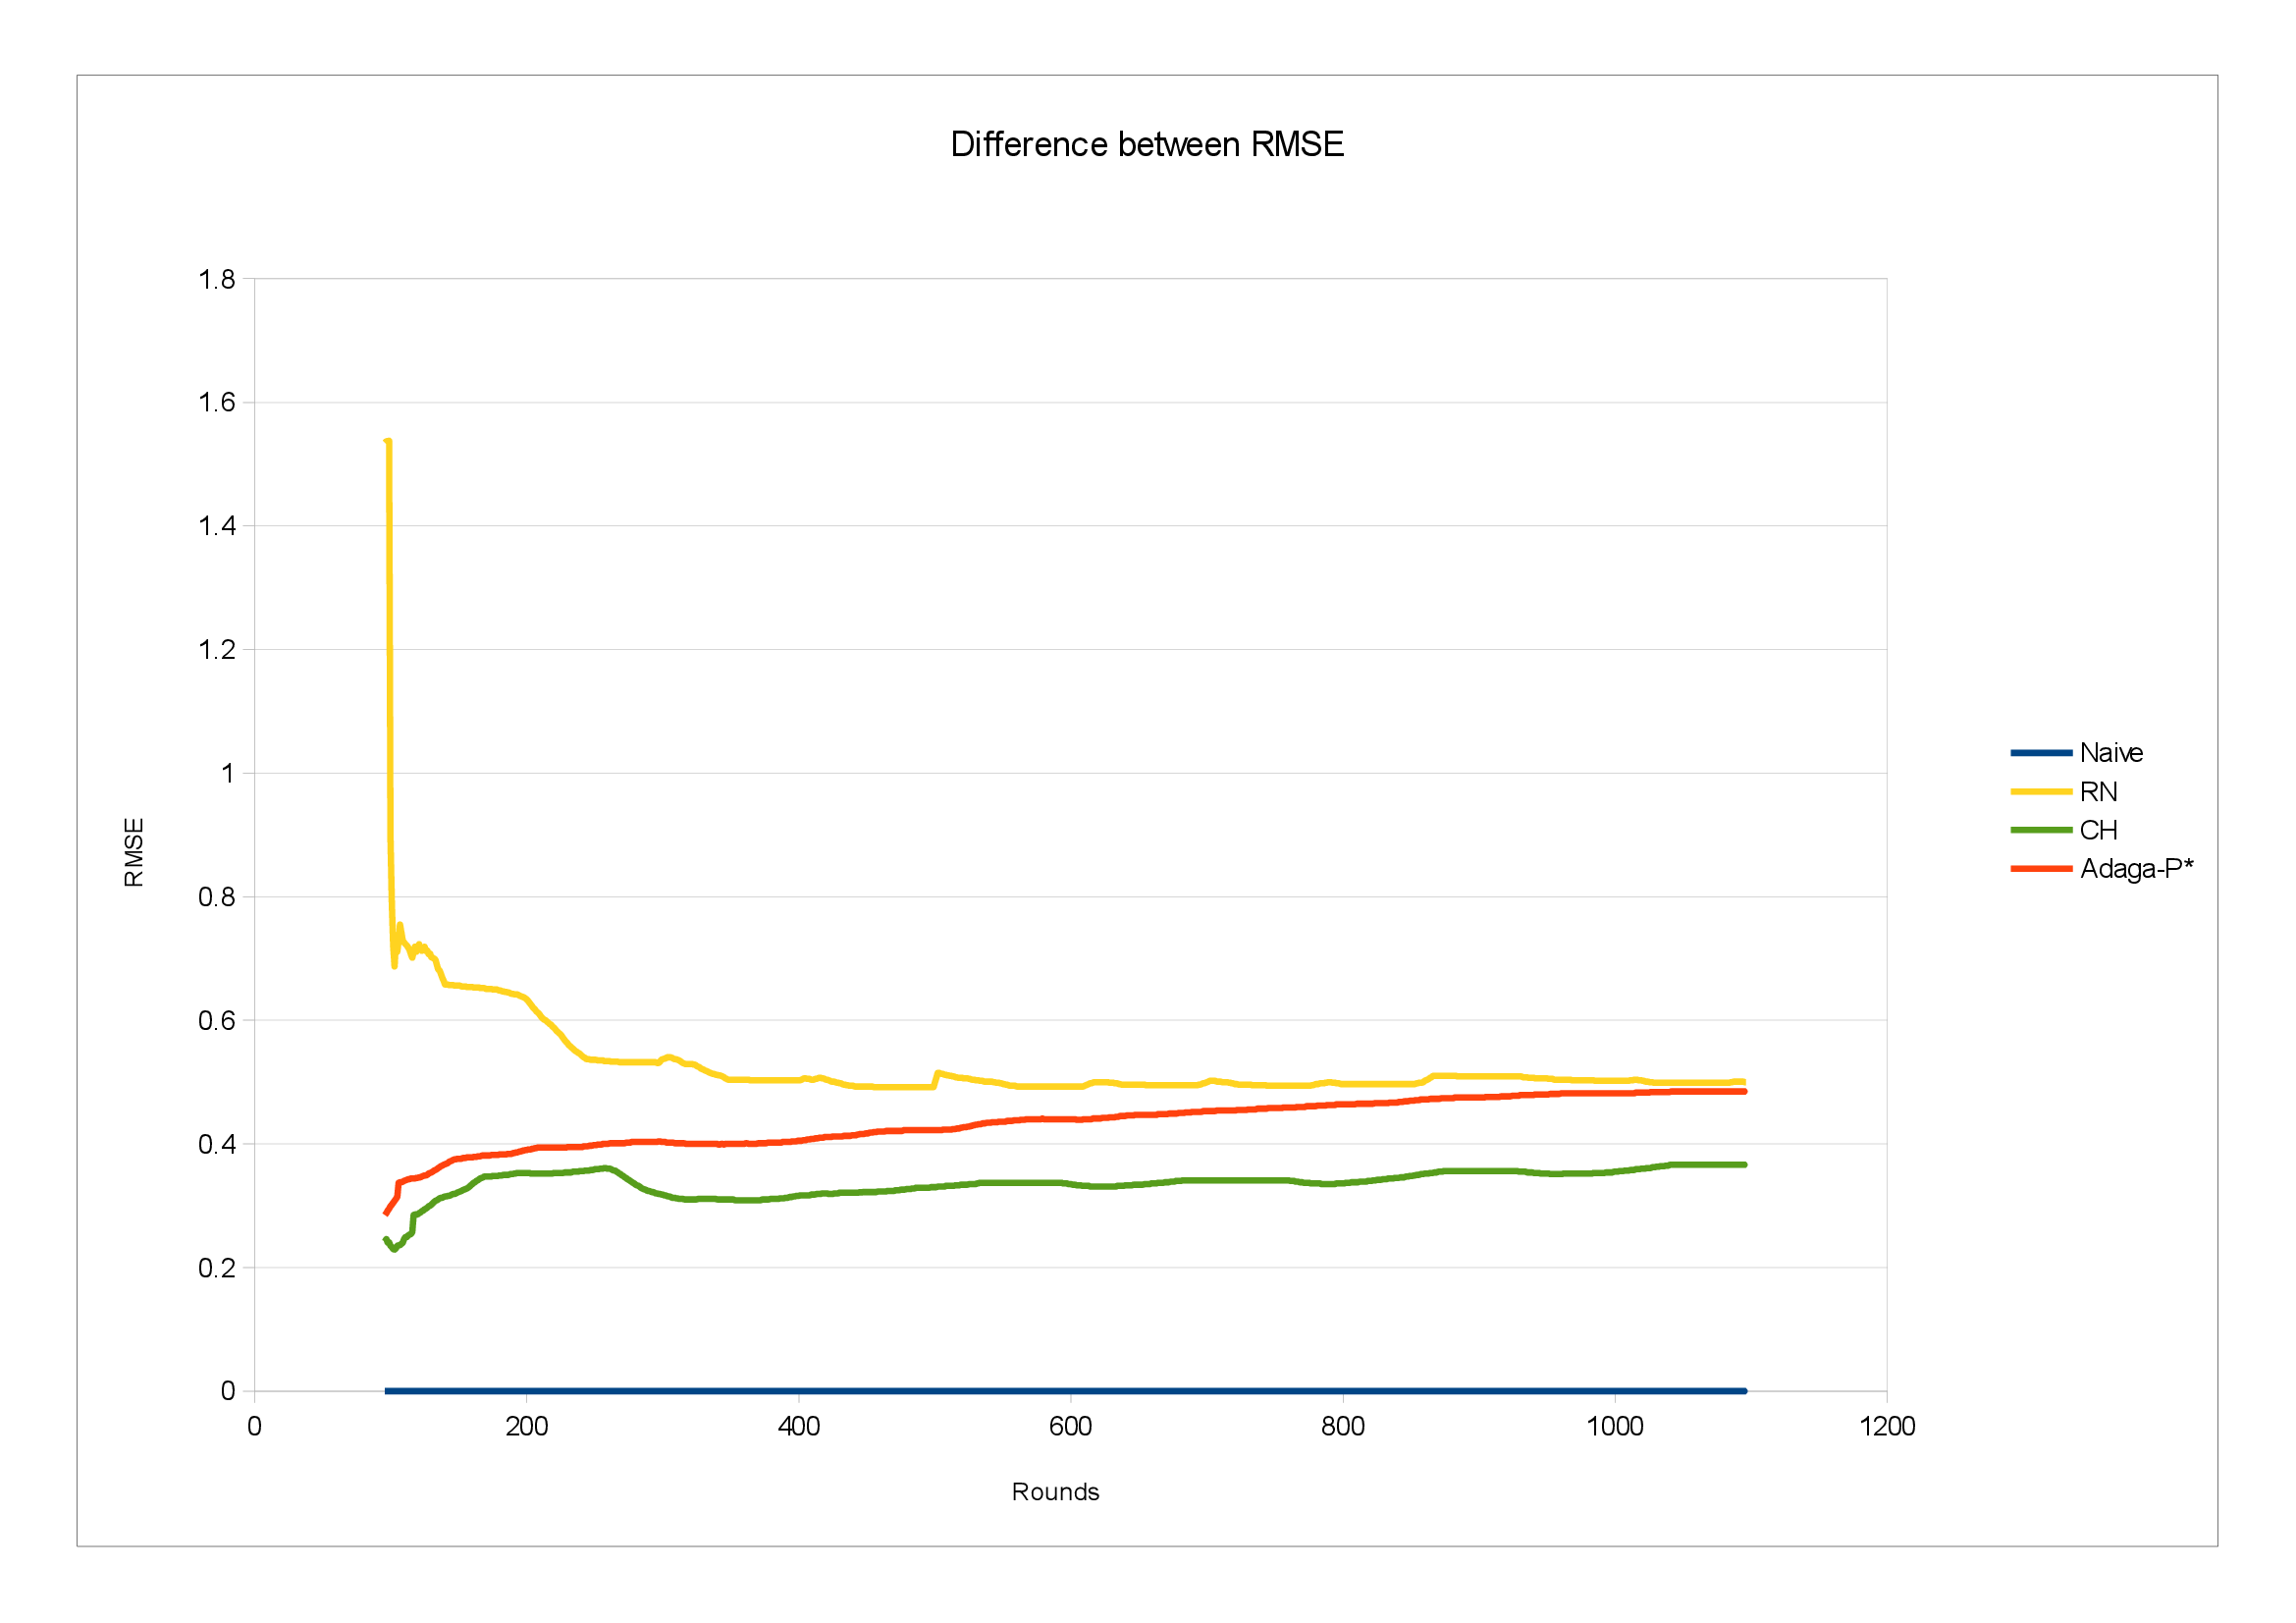
\includegraphics[scale=0.09]{graf_RMSE_.png}
    \caption{RMSE per Round}
    \label{fig:rmse}
\end{figure}

In the Fig. \ref{fig:num-msg}, one can observe a graph with the evolution of the
number of transmitted messages ({\it "NumMsg"} for short) in tested approaches.
NumMsg in the Naive approach grows linearly faster than in the other approaches.
As one can observe in Fig. \ref{fig:num-msg-without-naive}, the BCWSN-CH is
which has the lowest number of messages, followed by BCWSN-RN, and finally the
Adaga-P* approach.

\begin{figure}[!htb]
\centering
	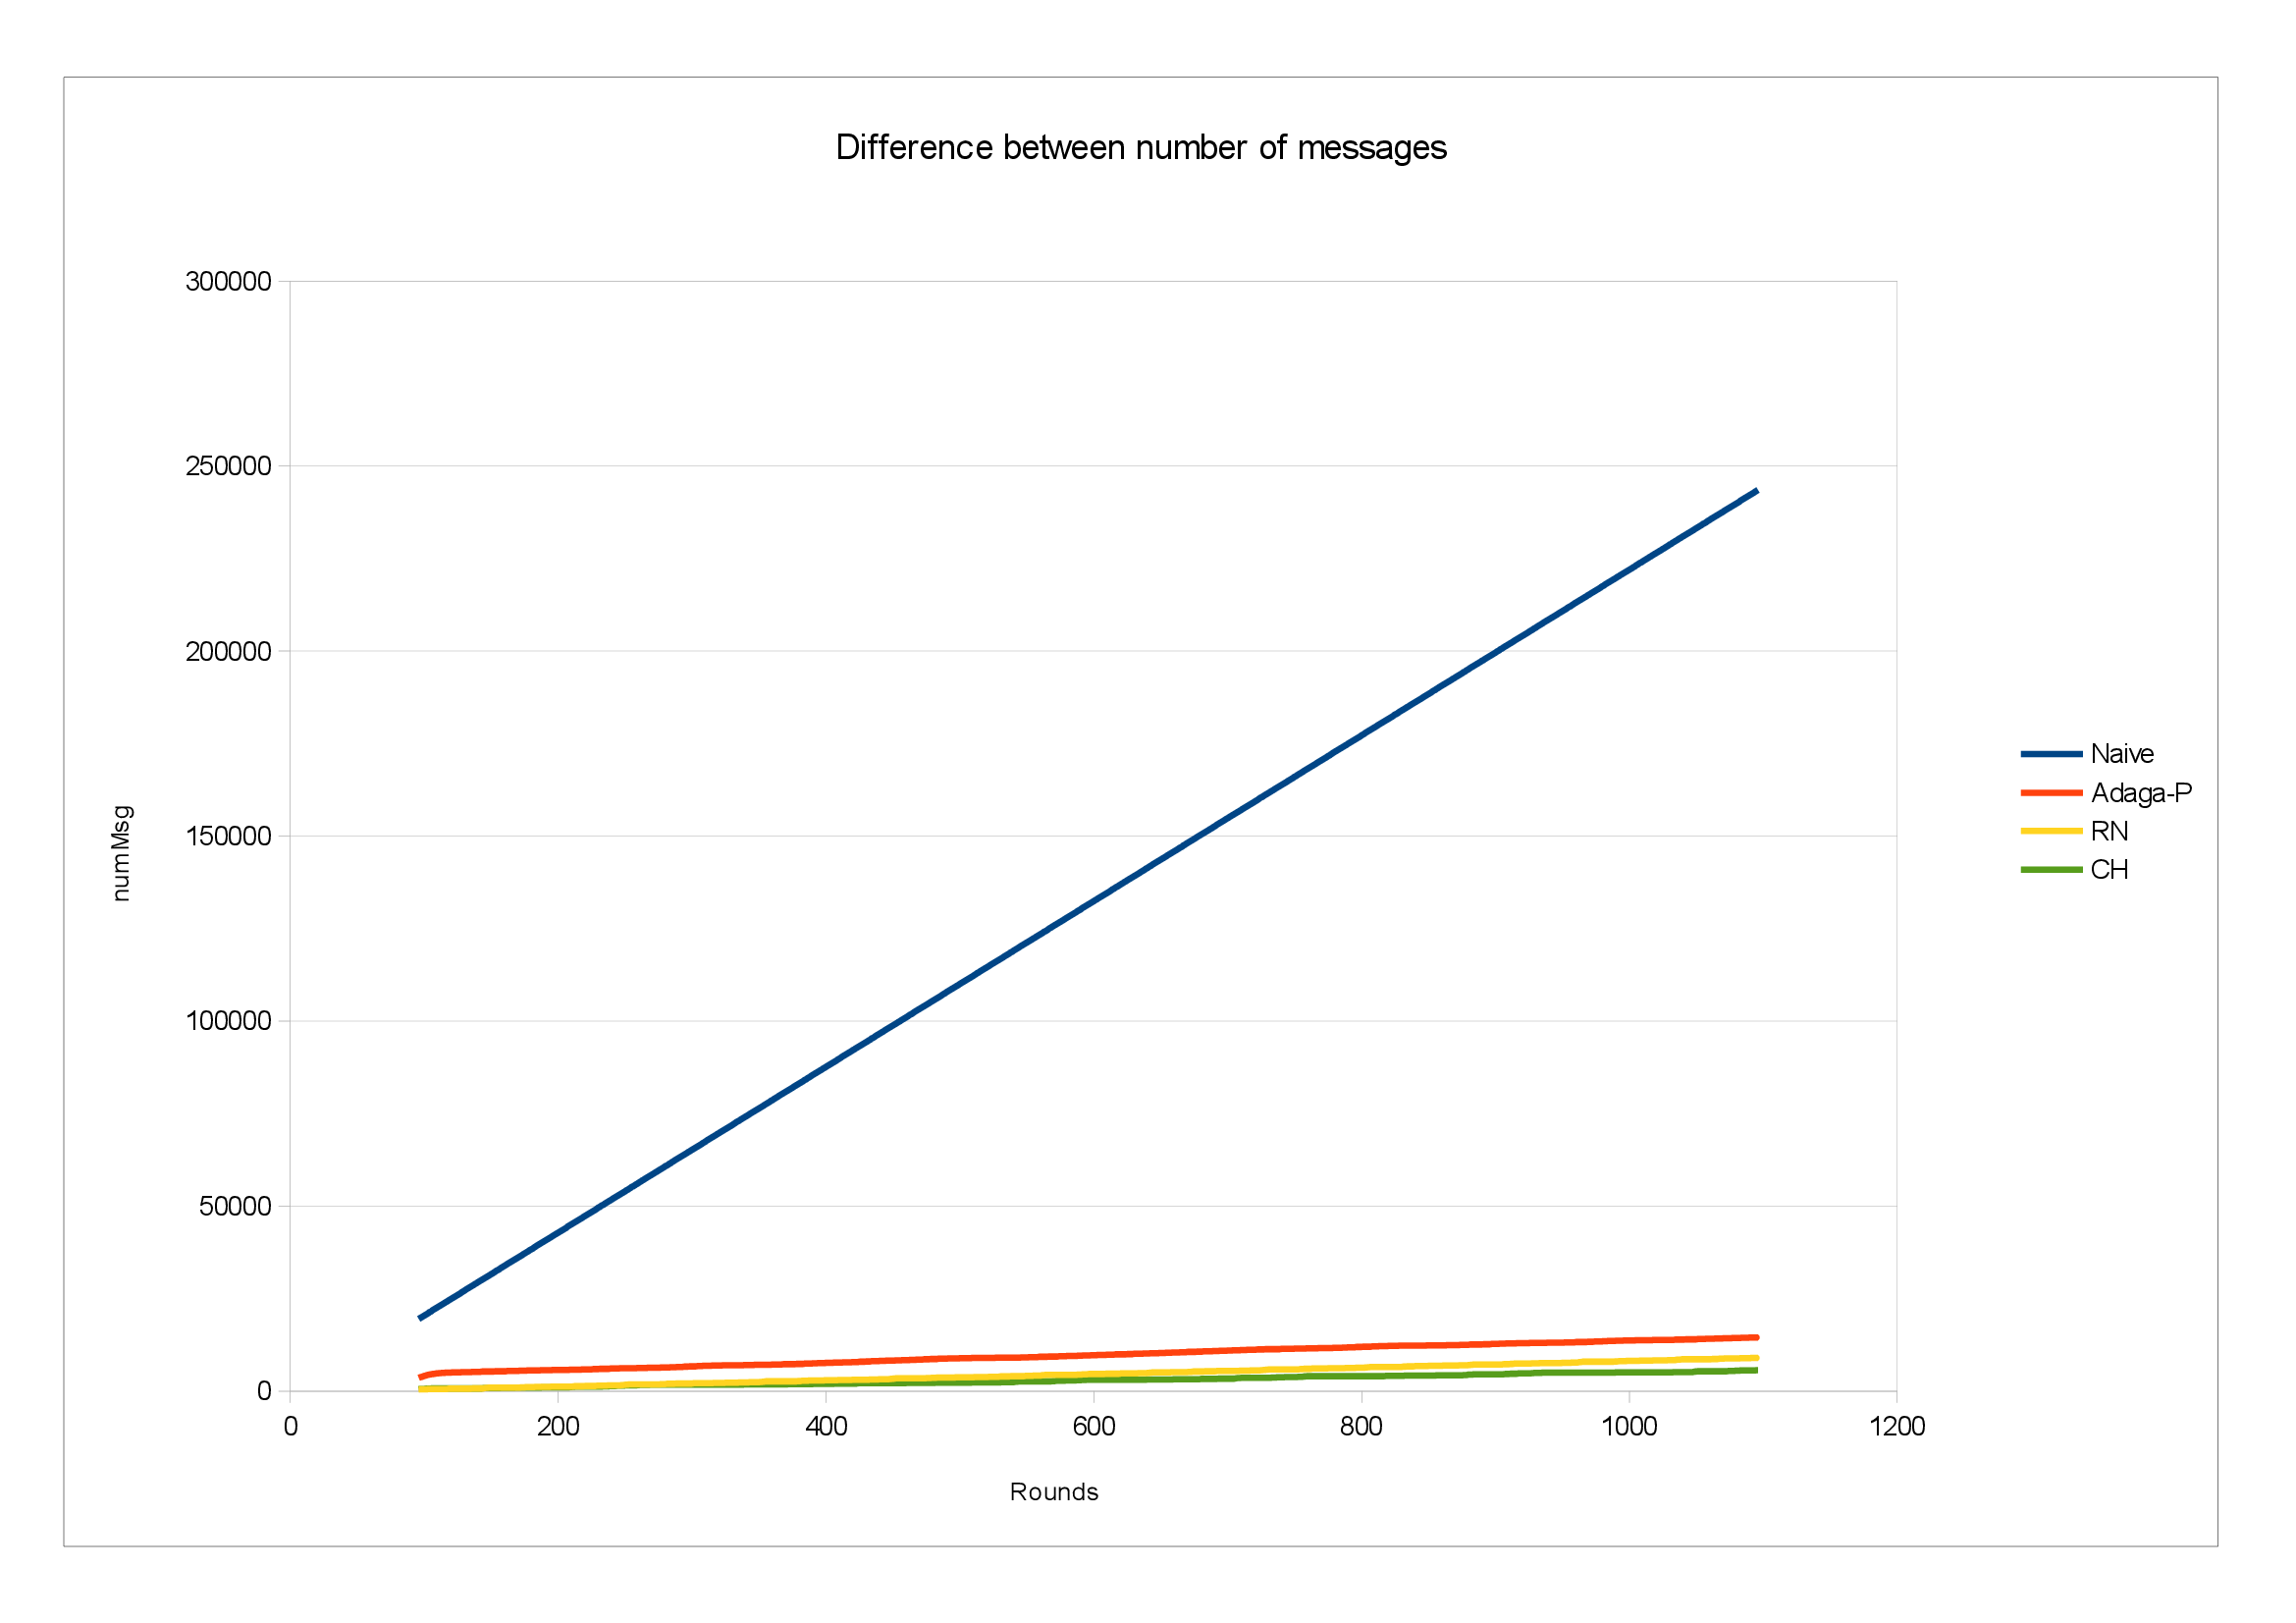
\includegraphics[scale=0.09]{graf_numMsg_.png}
    \caption{Number of Messages per Round}
    \label{fig:num-msg}
\end{figure}

\begin{figure}[!htb]
\centering
	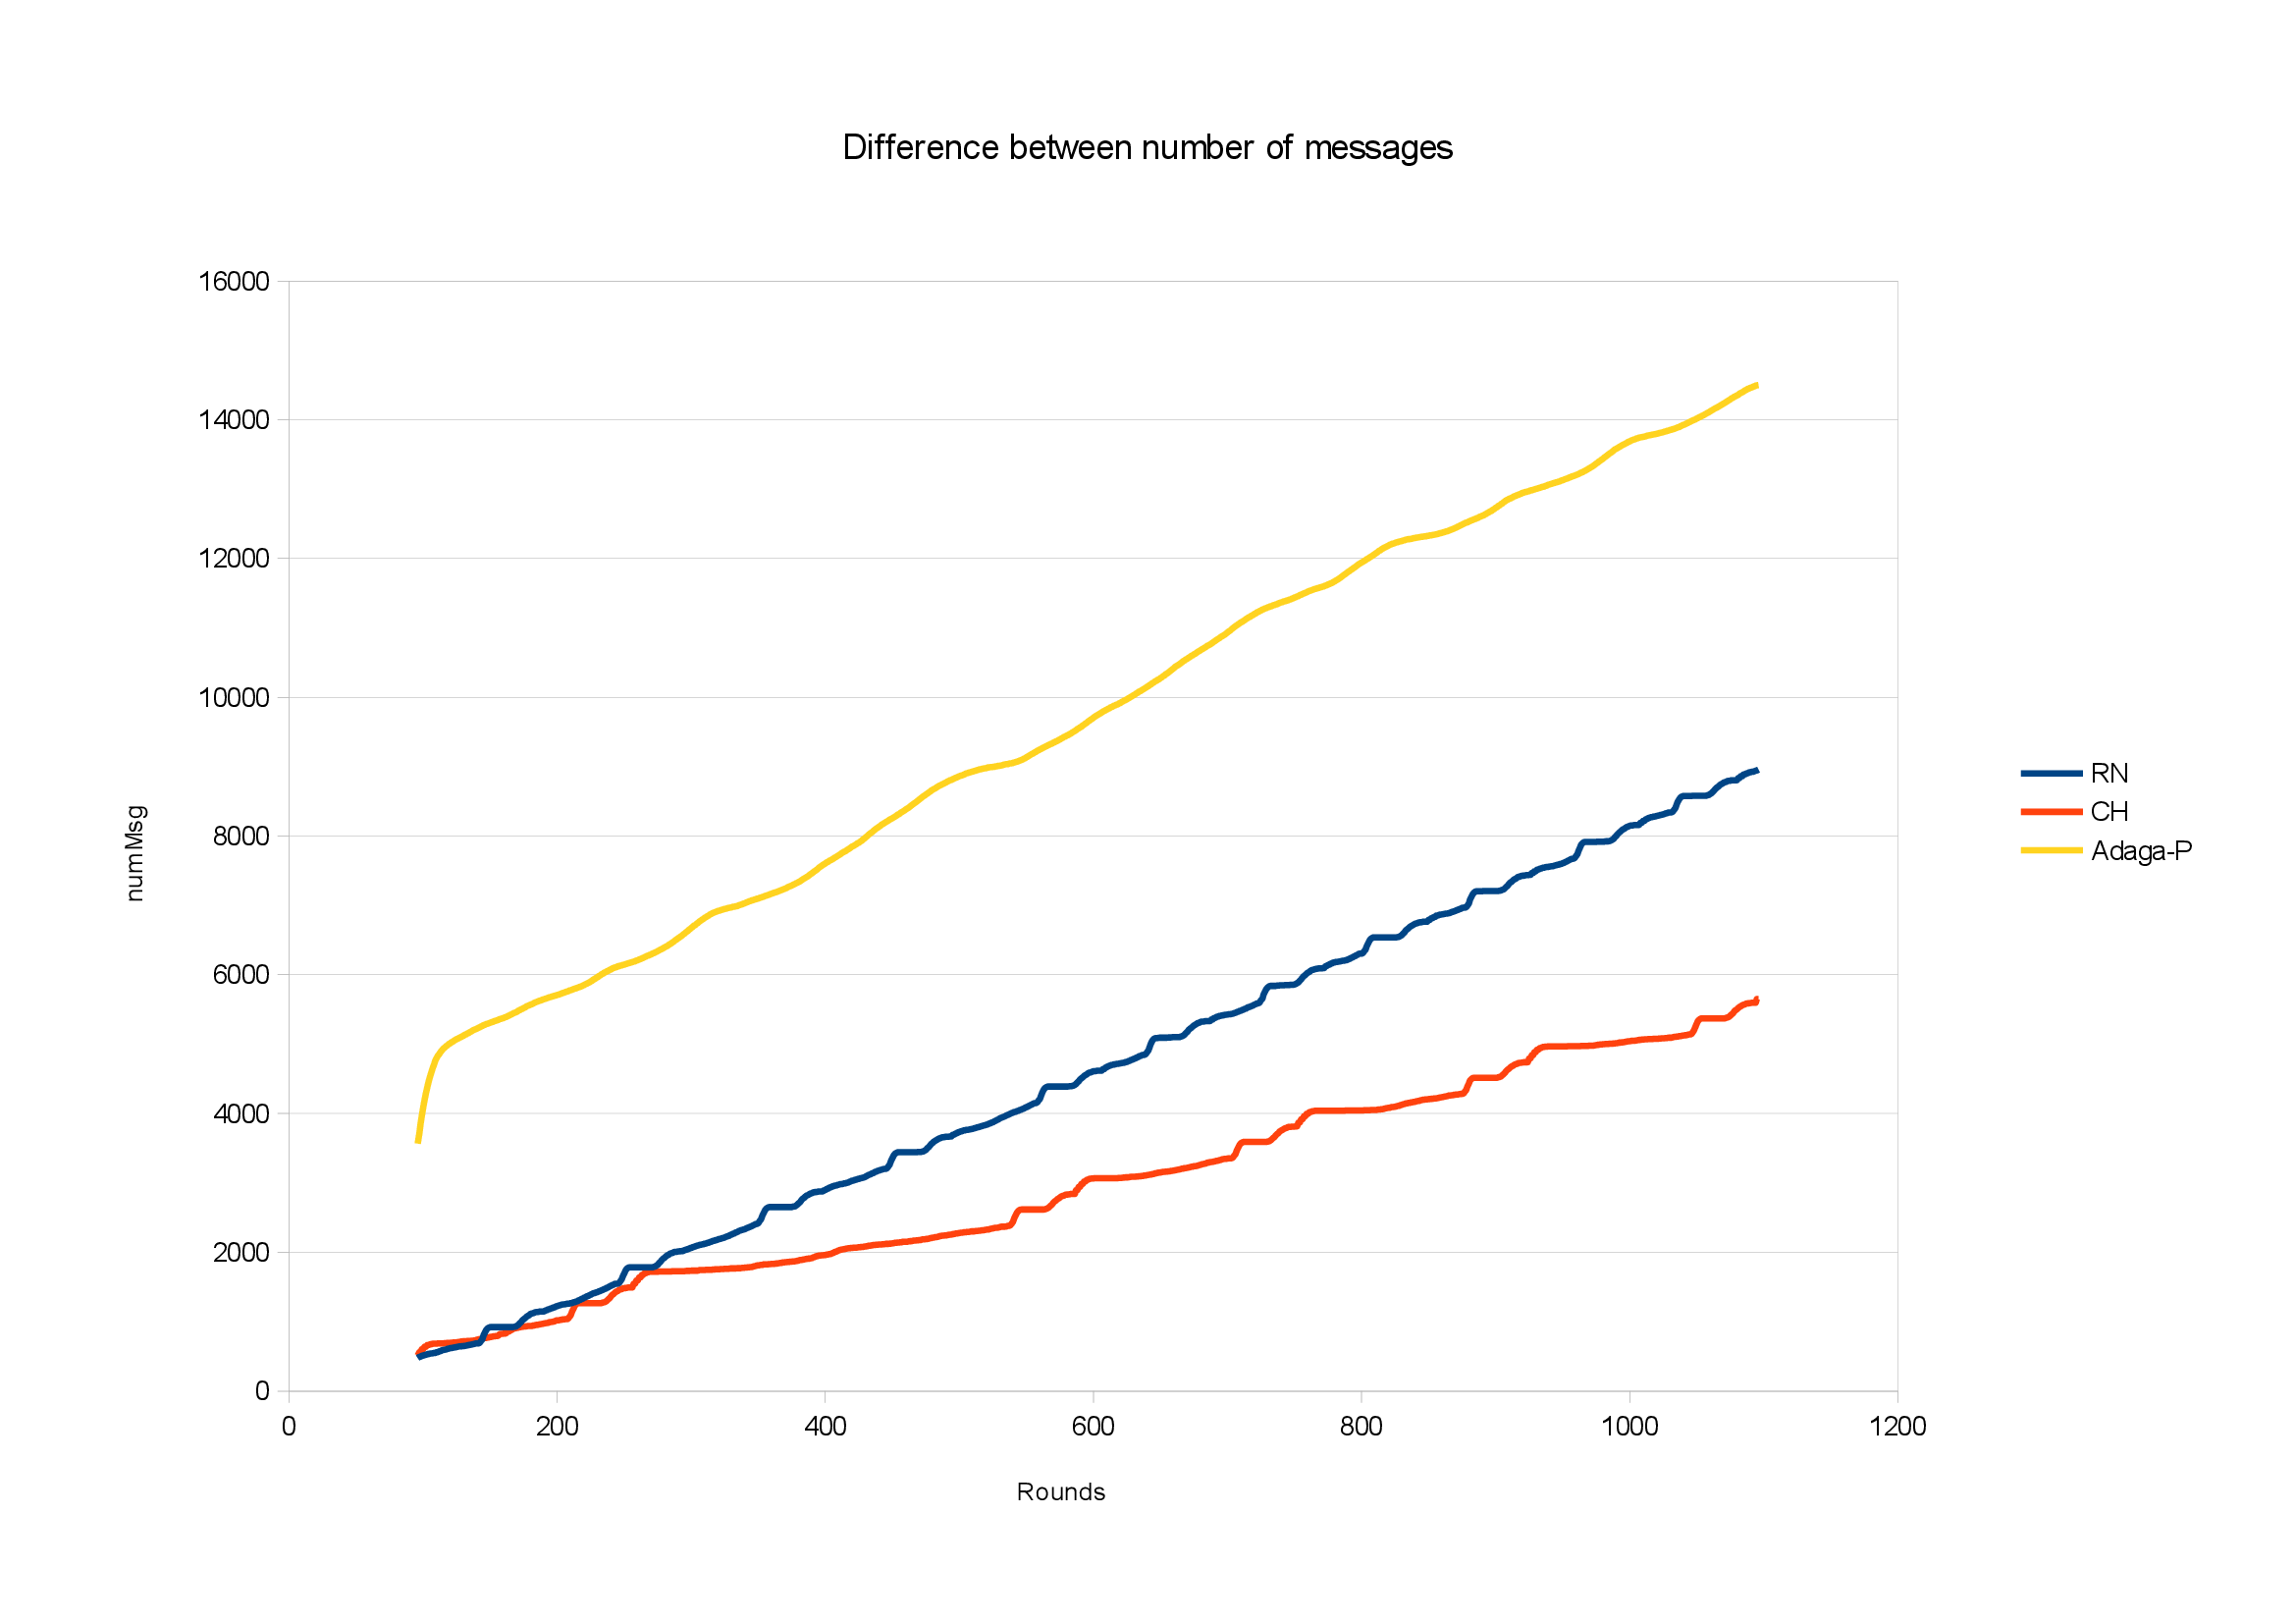
\includegraphics[scale=0.09]{graf_NumMsg_without_naive_.png}
    \caption{Number of Messages per Round without Naive}
    \label{fig:num-msg-without-naive}
\end{figure}

Finally, the graph in Fig. \ref{fig:sens-reading} shows the evolution of
the data sensed readings between the 4 tested approaches.
Naive and Adaga-P* approaches, as one can observe, have the same number of data
sensed readings (53) per round, because in these approaches all sensors
make sensing in all cycles. In the BCWSN-CH, sensors do not make sensing while
waiting to receive new coefficients after sending novelties to sink, and in the
BCWSN-RN, only the Representative Nodes (one per cluster) make sensing.

\begin{figure}[!htb]
\centering
	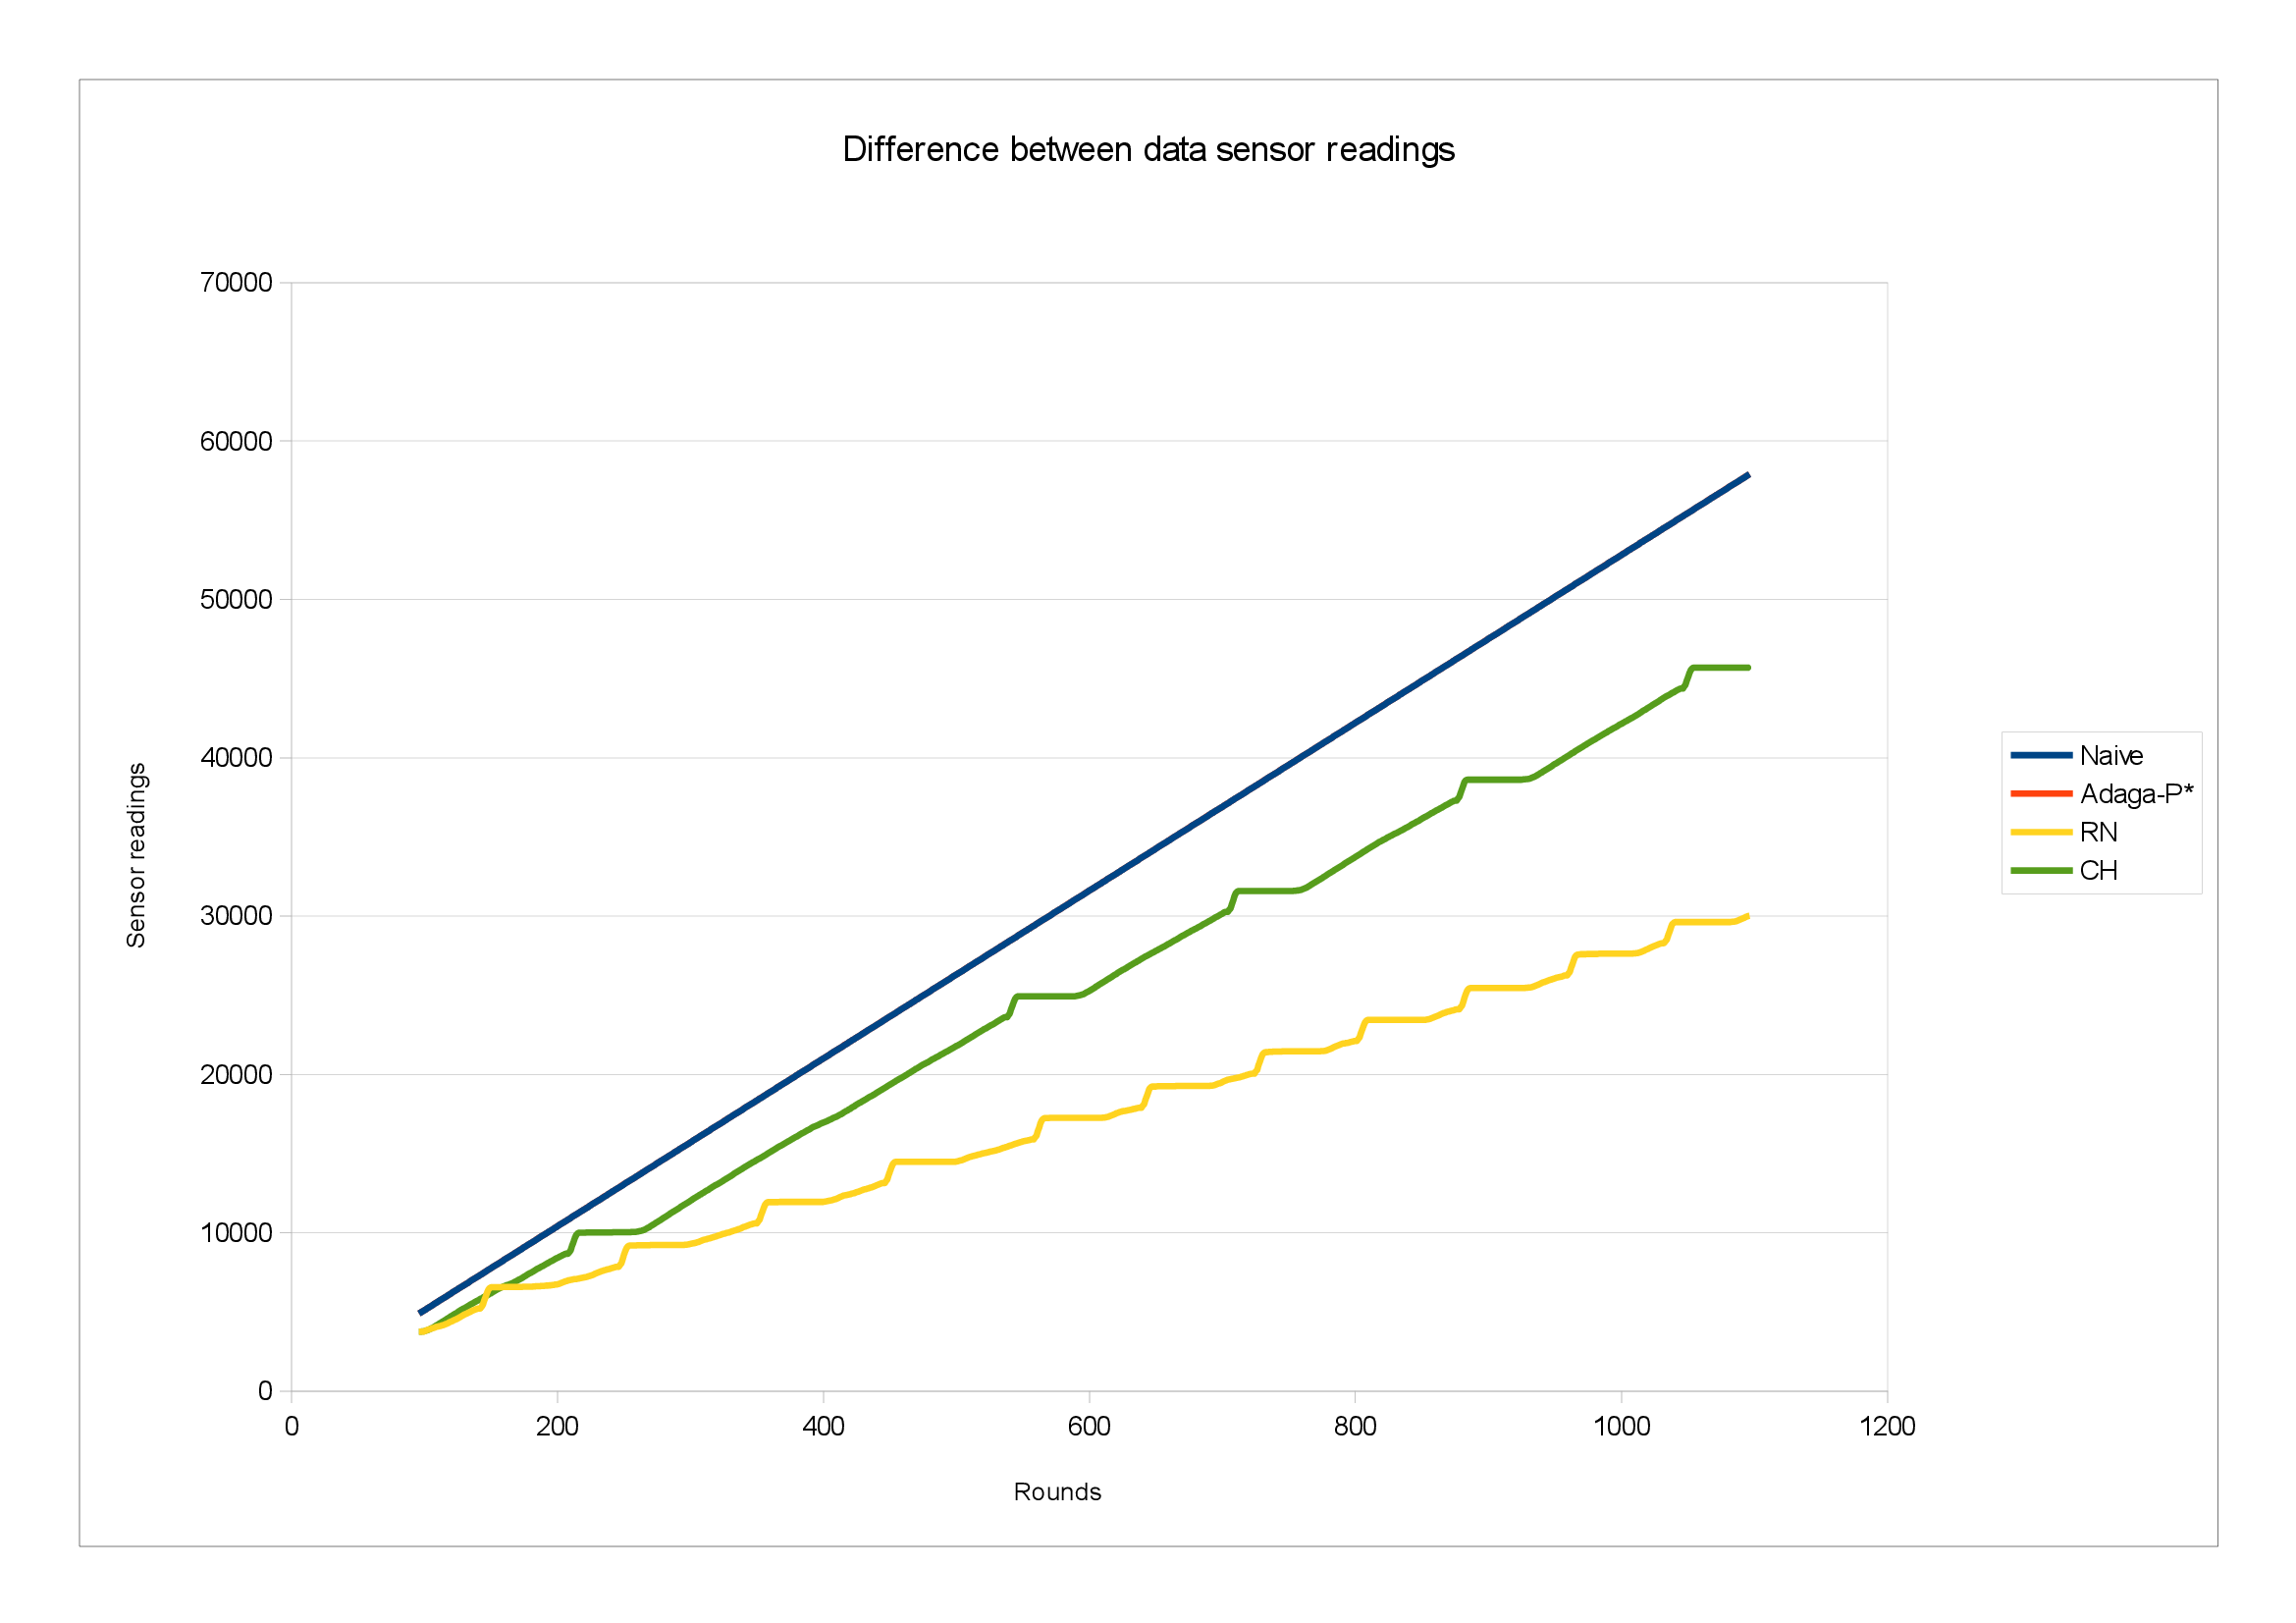
\includegraphics[scale=0.09]{graf_SREAD_.png}
    \caption{Number of Data Sensed Reading per Round}
    \label{fig:sens-reading}
\end{figure}


\section{Conclusion}

As result of our experiments, we show that the use of the \textit{Behavioral
Correlation} approach associated with a temporal correlation technique using two
different methods for intra-cluster scheduling, namely Representative Nodes
(RNs) or Cluster Heads (CHs), brought a great benefit to the energy economy of
Wireless Sensor Networks (WSNs), since, while it remained a low RMS Error for
the data obtained by the sink using such techniques (behavio-temporal
suppression), two important factors in energy expenditure of a sensor network
decrease, which are the total number of messages sent on the network and the
total number of sensor readings.


% conference papers do not normally have an appendix



\bibliographystyle{IEEEtran}
\bibliography{IEEEabrv,ISCC2014rodrigues_brayner_maia}  
% ISCC2014rodrigues_brayner_maia.bib is the name of the Bibliography in this case
% You must have a proper ".bib" file
%  and remember to run:
% latex bibtex latex latex
% to resolve all references

\end{document}


